\documentclass[sigconf,nonacm]{acmart}

\usepackage{balance}
\usepackage{booktabs}
\usepackage{float}
\usepackage{tabularx}
\usepackage{tikz}
\usepackage{listings}
\usepackage{xcolor}

\settopmatter{printacmref=false, printfolios=false}
\setlength{\emergencystretch}{1em}
\setlength{\textfloatsep}{10pt}
\raggedbottom
\lstdefinelanguage{sparql}{
  keywords={PREFIX, SELECT, WHERE, GRAPH, INSERT, DATA, DELETE, WITH, UNION, FILTER, BIND, VALUES, OPTIONAL, ORDER, BY, DESC},
  sensitive=true,
  morestring=[b]",
  morecomment=[l]\#
}
\lstset{
  language=sparql,
  basicstyle=\ttfamily\footnotesize,
  keywordstyle=\bfseries\color{blue!65!black},
  columns=fullflexible,
  keepspaces=true,
  breaklines=true,
  showstringspaces=false,
  frame=single,
  backgroundcolor=\color{black!3}
}

\begin{document}

\title{PluggedIn: A Semantic Web Approach to Electric Vehicle Charging Accessibility}
\titlenote{Project repository and implementation artifacts at \url{https://github.com/chohoon901/PluggedIn}.}

\author{Jungwon Youn}
\affiliation{\institution{University of Victoria}\city{Victoria}\country{Canada}}
\email{jungwonyoun@uvic.ca}

\author{Sunghun Cho}
\affiliation{\institution{University of Victoria}\city{Victoria}\country{Canada}}
\email{shcho980901@uvic.ca}

\author{Elias Dockal}
\affiliation{\institution{University of Victoria}\city{Victoria}\country{Canada}}
\email{eliasdockal@uvic.ca}

\begin{abstract}
Electric vehicle charging records combine locations, connector types, operating periods, network memberships, and equipment specifications from different sources. PluggedIn models these records with an OWL ontology and loads a 20-station Vancouver-area sample into an authenticated OpenLink Virtuoso graph. The migration verifies 193 relational records, and the application uses Virtuoso for station search and profile management. Four SPARQL competency queries demonstrate network membership, minimum DC power, direct connector matches, and directional adapter candidates. Two are available as dedicated application screens. The project code, data and setup instructions are available at \url{https://github.com/chohoon901/PluggedIn}.
\end{abstract}

\keywords{Semantic Web, RDF, OWL, SPARQL, electric vehicle charging}
\maketitle

\section{Problem and Competency Questions}

A driver needs to know where a particular vehicle can connect and whether the available evidence supports charging at the planned arrival time. The prototype integrates station, port, and operator information from a matched NLR--Open Charge Map sample. It combines these facts with separately registered vehicles, drivers, and network memberships. The graph supports the following four questions.

\begin{itemize}
  \item \textbf{CQ1.} Which stations belong to a specified network, and where are they located?
  \item \textbf{CQ2.} Which DC charging ports have recorded power ratings or published equipment ratings that meet a user-supplied minimum power threshold, and which connectors do they use?
  \item \textbf{CQ3.} Which ports at Vancouver stations match the connectors directly accepted by registered vehicles?
  \item \textbf{CQ4.} Which catalogue adapters connect a station port to an inlet of the selected vehicle?
\end{itemize}

The search page also evaluates operating hours, site access, direct connection, and payment at the chosen arrival time. The app displays \emph{Needs review} when the available evidence is insufficient for an overall decision.

\section{Ontology and Relational Mapping}

We authored the TBox in Prot\'eg\'e and exported \texttt{PluggedIn.rdf} as RDF/XML. The model uses RDF, RDFS, OWL and XML Schema. It uses \texttt{plug:} for the project IRI followed by \texttt{ontology/}, and \texttt{mig:} for the project IRI followed by \texttt{migration/}. The project IRI is \url{https://github.com/chohoon901/PluggedIn/}.

The TBox declares 12 OWL classes, 11 object properties and 40 datatype properties. The ER model's specialization hierarchy is preserved through \texttt{rdfs:subClassOf}, with \texttt{Network}, \texttt{Operator} and \texttt{SiteOwner} as subclasses of \texttt{Organization}. The one-to-many relationships between stations and their ports or operating periods are represented by the object properties \texttt{hasPort} and \texttt{hasOperatingPeriod}. The many-to-many relationship between vehicles and connector types is represented by \texttt{vehicleAccepts}. A station carries decimal latitude and longitude directly. An operating period uses day, opening time and closing time strings, with time-zone and evidence information stored separately in the graph. \texttt{Adapter} has directed links from the station-side connector to the vehicle-side connector.

\begin{table}[t]
\caption{Examples from the relational-to-RDF mapping.}
\label{tab:mapping}
\small
\begin{tabularx}{\columnwidth}{@{}>{\raggedright\arraybackslash}p{.34\columnwidth}>{\raggedright\arraybackslash}X@{}}
\toprule
Relational concept & RDF representation \\
\midrule
Row and primary key & A typed individual with a dataset-scoped IRI derived from the key. \\
Station and organization roles & \texttt{partOfNetwork}, \texttt{operatedBy} and \texttt{ownedBy}. Role classes share the corresponding organization resource. \\
Port and operating-period foreign keys & Station edges \texttt{hasPort} and \texttt{hasOperatingPeriod}. A port also uses \texttt{hasConnectorType}. \\
Vehicle--connector association & A \texttt{mig:VehicleAcceptance} record preserves the association key. The \texttt{vehicleAccepts} edge supports direct queries. \\
Driver and membership & \texttt{hasMembership} connects a driver to a membership, which \texttt{belongsToNetwork}. \\
Typed attributes & \texttt{powerKw} uses \texttt{xsd:decimal} and \texttt{acceptsGuestPayment} uses \texttt{xsd:boolean}. \\
\bottomrule
\end{tabularx}
\end{table}

The exporter maps 13 tables and 65 columns. The extra association resource is defined by the mapping vocabulary, so the table count and TBox class count have different meanings. For example, \texttt{data/sample20/Station/1} resolves under the project IRI and identifies the BC Hydro DoubleTree location. Unlike relational constraints, RDFS domain and range declarations describe semantic relationships rather than enforcing database-style integrity. Under the Open World Assumption, missing triples do not necessarily imply false statements. Therefore, unique profile identifiers, required fields, and referential integrity are enforced at the application level, while missing evidence is treated as unknown.

\section{Graph Population and Updates}

The \texttt{sample20} build joins NLR station identifiers to Open Charge Map provider references and preserves the source rows and their provenance. The bundled SQLite snapshot includes 20 stations, 26 ports, 98 operating periods, 2 synthetic drivers, 4 synthetic vehicles and 6 synthetic memberships. The migration imports the snapshot and station metadata into the named graph at the project IRI plus \texttt{graph/app/}. It checks that anonymous queries cannot read the graph and verifies all 193 source records and the mapped relationships before marking the graph ready. SQLite supplies the read-only migration input.

A separate SPARQL update adds four sourced adapter entries and published equipment evidence. Kaslo's 250 kW value is the operator's published charging-group maximum~\cite{tesla}. Prism Engineering documents 50 kW installed DC chargers at Norgate Park~\cite{prism}. The RDF update records evidence scopes and links alongside the numbers. Open Charge Map's connector-derived estimates are retained in the source manifest. The other three DC sites lack a verified rating in this sample.

Drivers, vehicles and memberships are added, edited and deleted through application forms. The data access layer translates the validated change set into scoped SPARQL updates~\cite{update}. It checks the expected graph revision before committing a write. Listing~\ref{lst:dml} illustrates the corresponding insert, edit and delete operations using a synthetic driver in a scratch graph.

\begin{lstlisting}[caption={SPARQL write example for a scratch graph.},label={lst:dml}]
PREFIX plug: <https://github.com/chohoon901/PluggedIn/ontology/>
PREFIX d: <urn:pluggedin:report:>
INSERT DATA {
  GRAPH d:demo {
    d:driver a plug:Driver ;
      plug:licenceNumber "DEMO-RDF" ;
      plug:driverName "Sample driver" .
  }
};
WITH d:demo
DELETE { d:driver plug:driverName ?old . }
INSERT { d:driver plug:driverName "Edited driver" . }
WHERE  { d:driver plug:driverName ?old . };
DELETE WHERE { GRAPH d:demo { d:driver ?p ?o . } }
\end{lstlisting}

\section{SPARQL Queries and Observed Results}

The complete \texttt{SELECT} statements are in \texttt{sparql\_queries.rq}. Each query is evaluated against the configured application graph using SPARQL 1.1~\cite{query}. The repository uses explicit graph patterns and filters. Table~\ref{tab:results} summarizes results from the migrated sample.

\begin{table}[t]
\caption{Results verified on the application graph. CQ2 counts rows by port, and CQ4 counts port--adapter candidates per vehicle.}
\label{tab:results}
\small
\begin{tabularx}{\columnwidth}{@{}>{\raggedright\arraybackslash}p{.21\columnwidth}>{\raggedright\arraybackslash}X@{}}
\toprule
Query & Observed result \\
\midrule
CQ1 & 1 station for \texttt{BCHYDRO}, North Vancouver District DoubleTree, at 49.31281722, $-123.0278656$. \\
CQ2, 50 kW & 3 rows at 2 sites. Kaslo has a 250 kW result and Norgate Park has two 50 kW connector rows. \\
CQ2, 250 kW & 1 row for Kaslo. At 251 kW the result is empty. \\
CQ3 & 8 direct-connection rows for stations in Vancouver. \\
CQ4 & 4, 1, 2 and 16 rows for the CHAdeMO, J1772, J1772COMBO and Tesla sample vehicles, respectively. \\
\bottomrule
\end{tabularx}
\end{table}

\paragraph{CQ1 and CQ3.}
CQ1 matches the network's organization name and returns the station, coordinates and optional operator name. It treats the charging network and station operator as separate roles. The following projection illustrates the network query with \texttt{app:} bound to the application graph IRI.

\noindent\begin{minipage}{\columnwidth}
\begin{lstlisting}[caption={CQ1 network membership and coordinates.},label={lst:network}]
SELECT ?stationName ?lat ?lon ?operatorName
WHERE { GRAPH app: {
  ?s a plug:Station ; plug:partOfNetwork ?n ;
     plug:latitude ?lat ; plug:longitude ?lon .
  ?n plug:orgName ?networkName .
  FILTER (STR(?networkName) = "BCHYDRO")
  OPTIONAL { ?s plug:stationName ?stationName . }
  OPTIONAL {
    ?s plug:operatedBy/plug:orgName ?operatorName .
  }
} }
\end{lstlisting}
\end{minipage}

CQ3 joins Vancouver station ports and the connectors accepted by each vehicle. It matches normalized connector names and verified current types for J1772/AC, CCS1/DC and CHAdeMO/DC. Virtuoso returns the vehicle, station and port for each matching pair.

\paragraph{CQ2.}
Fast Charging passes the minimum to the query in Listing~\ref{lst:power}. It uses a port rating when available and published equipment evidence otherwise. The results show the station, connector, rating scope and source.

\begin{lstlisting}[caption={Power and current conditions inside the CQ2 graph pattern.},label={lst:power}]
VALUES ?minimumPowerKw { 50 }
?station a plug:Station ; plug:hasPort ?port .
?port plug:currentType ?currentType ;
  plug:hasConnectorType/plug:connectorName
    ?connectorName .
{
  ?port plug:powerKw ?powerKw .
  BIND("Port rating" AS ?scope)
}
UNION {
  ?port (mig:operatorPublishedPowerKw|
         mig:installedChargerPowerKw) ?powerKw ;
    mig:powerEvidenceScope ?scope ;
    mig:powerEvidenceSource ?source ;
    mig:powerEvidenceCheckedOn ?checked .
  FILTER NOT EXISTS { ?port plug:powerKw ?rating }
}
FILTER (STR(?currentType) = "DC" &&
        ?powerKw >= ?minimumPowerKw)
\end{lstlisting}

\paragraph{CQ4.}
Adapter Finder uses the selected vehicle's IRI. It compares the port's connector family with the adapter's \texttt{fromConnector} family and the vehicle inlet with its \texttt{toConnector} family. When both current types are known, they must agree. A direct match to any of the vehicle's inlets suppresses the adapter candidate for that port. For instance, the sample J1772COMBO vehicle returns a Ford NACS-to-CCS1 candidate at Kaslo. These candidates represent connector compatibility evidence. Vehicle model and charging network eligibility require their own checks.

\balance
\section{Application and Reproduction}

\begin{figure}[H]
\centering
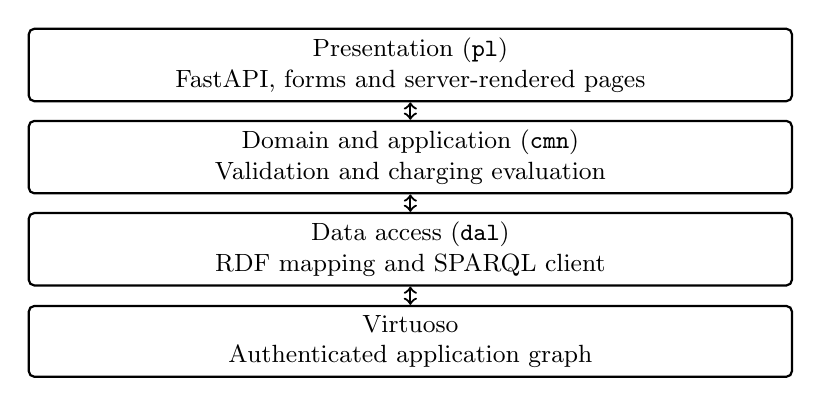
\begin{tikzpicture}[
  layer/.style={draw, rounded corners=2pt, align=center,
    text width=.78\columnwidth, minimum height=6mm, font=\small},
  every path/.style={thick}]
  \node[layer] (ui) at (0,0) {Presentation (\texttt{pl}) \\ FastAPI, forms and server-rendered pages};
  \node[layer] (domain) at (0,-1.17) {Domain and application (\texttt{cmn}) \\ Validation and charging evaluation};
  \node[layer] (dal) at (0,-2.34) {Data access (\texttt{dal}) \\ RDF mapping and SPARQL client};
  \node[layer] (store) at (0,-3.51) {Virtuoso \\ Authenticated application graph};
  \draw[<->] (ui) -- (domain);
  \draw[<->] (domain) -- (dal);
  \draw[<->] (dal) -- (store);
\end{tikzpicture}
\caption{Local runtime architecture. The data access layer also handles the one-time SQLite-to-RDF import.}
\Description{Four vertically connected boxes show the path from web pages through domain services and RDF data access to the Virtuoso graph.}
\label{fig:architecture}
\end{figure}

The normal runtime connects FastAPI to Virtuoso through a data access layer. Station search and profile forms call the application services. Fast Charging and Adapter Finder send SPARQL queries to the same graph that stores the vehicle and membership records. The named graph uses an application account via \texttt{/sparql-auth}. Teammates can recreate the sample in their own local Virtuoso instances.

The repository quickstart specifies the graph configuration and credentials. The Windows quickstart takes \texttt{-Migrate} for a new graph and \texttt{-CheckOnly} for verification. On either platform the project Python environment can run the migration module directly. With the Virtuoso account configured in the environment, run the following from \texttt{project/}.

\begin{lstlisting}[language=bash, caption={Base RDF/XML export and verification of an existing application graph.}]
python -m ca.uvic.ecs.csc501.dal.scripts.export_rdf \
  --dataset sample20 --output sample20-data.rdf
python -m ca.uvic.ecs.csc501.dal.scripts.migrate_to_virtuoso --check
\end{lstlisting}

The export produces the base ABox in RDF/XML. Run the migration module without \texttt{--check} for a first import into an empty app graph. The migration reads the bundled snapshot and installs the application records and equipment evidence. The file \texttt{sample20\_equipment\_evidence.ru} contains the equipment additions. The \texttt{--sample-equipment} option applies these additions to an existing app graph.

A repeatable station-search demonstration uses the synthetic member and J1772 vehicle with arrival at 12:00 Pacific time on 2 November 2026. It returns 20 stations with 1 Available and 19 Needs review. The available location is SWTCH Energy at 5965 Student Union Blvd. Profile create, edit and delete operations were verified against Virtuoso, and the sample charging and adapter screens read the resulting graph-backed data.

\section{Conclusion}

PluggedIn preserves source identifiers, typed attributes, relationships and uncertainty when migrating a relational sample into RDF. The same graph supports application writes and four reproducible competency queries. Explicit provenance lets the output search show published ratings alongside their scopes, while the adapter query leaves eligibility decisions to the relevant vehicle and network evidence.

\section*{AI Assistance}
OpenAI Codex assisted with comparing the report to the implementation, revising the text, and verifying the query results reported here~\cite{codex}.

\begin{thebibliography}{6}
\bibitem{query} Steve Harris and Andy Seaborne, editors. 2013. \emph{SPARQL 1.1 Query Language}. W3C Recommendation. \url{https://www.w3.org/TR/sparql11-query/}.
\bibitem{update} Paula Gearon, Alexandre Passant, and Axel Polleres, editors. 2013. \emph{SPARQL 1.1 Update}. W3C Recommendation. \url{https://www.w3.org/TR/sparql11-update/}.
\bibitem{prism} Prism Engineering. \emph{District of North Vancouver: EV Design and Implementation}. Consulted 20 November 2026. \url{https://www.prismengineering.com/projects/district-of-north-vancouver-ev-design-and-implementation/}.
\bibitem{tesla} Tesla. \emph{Vancouver, BC --- Kaslo St Supercharger}. Equipment rating recorded 19 November 2026. \url{https://www.tesla.com/en_CA/findus/location/supercharger/13658}.
\bibitem{codex} OpenAI. 2026. \emph{Codex}. AI-assisted report revision and local verification, 20 November 2026. \url{https://openai.com/codex/}.
\end{thebibliography}

\end{document}
